\scanpage{107}

Factorization of entire functions.

\margin{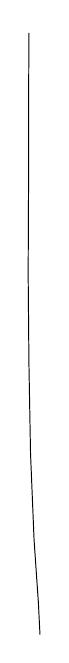
\begin{tikzpicture}[x=0.005cm,y=-0.005cm,baseline={(0,0)}]
\draw[line width=0.35pt] (19,13) -- (18,210) -- (18,400) -- (17,625) -- (19,855) -- (23,1080) -- (32,1300) -- (43,1460) -- (47,1540);
\end{tikzpicture}}
\uline{Theorem 1} (Weierstrass) Let $f(z)$ be an entire function, $(a_n)$ the sequence of its zeros, arranged in order \unsure{in|of} increasing moduli. Suppose $f(0)\ne0$. It is possible to find an increasing sequence of integers $\geq0$ $p_n$, and an entire function $g(z)$, such that one has

\[
 f(z)=e^{g(z)}\prod_n\left(1-\frac{z}{a_n}\right)e^{\frac{z}{a_n}+\frac{z^2}{2a_n^2}\unsure{+}\mathord{\cdot}\mathord{\cdot}\frac{z^{p_n}}{p_n a_n^{p_n}}} \tag*{(1)}
\]

the product being uniformly absolutely convergent when $z$ ranges over any bounded region. If \deleted{in addition} \inserted{a sequence of integers} $p_n$ satisfies

\[
 \sum\left|\frac{r}{a_n}\right|^{(p_n+1)}<+\infty\qquad\text{for any }r,
\]

then one can use this sequence in the expression \uline{1}. In particular, suppose $k$ an integer such that $\sum\frac{1}{|a_n|^{k+1}}<+\infty$, then one can take $p_n\deleted{\unsure{=|k}}\unsure{=}p$ for \deleted{every} $n$, with $p\leq k$ whence

\[
 f(z)=e^{g(z)}\prod_n\left(1-\frac{z}{a_n}\right)e^{\frac{z}{a_n}+\unsure{-|\cdots}+\frac{z^k}{ka_n^k}} \tag*{(2)}
\]

\margin{108}
